\documentclass[tikz,border=2pt]{standalone}
\usepackage{amsmath,amssymb}
\usepackage{tikz}
\usetikzlibrary{arrows.meta}

\begin{document}
% A linear map sends the grid to a grid: the unit square spanned by e1, e2 becomes the
% parallelogram spanned by f(e1), f(e2), the origin stays put, lines stay lines.
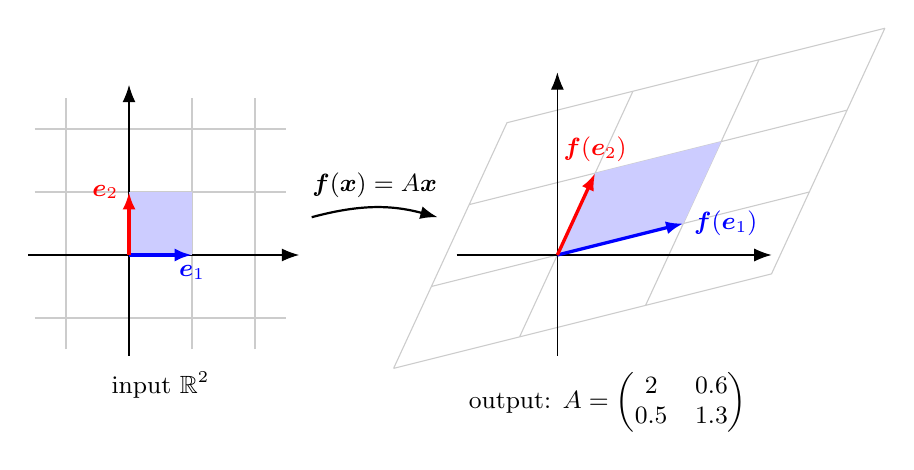
\begin{tikzpicture}[scale=0.8, every node/.style={font=\small}, >={Latex[length=2.2mm]}]
	\begin{scope}
		\draw[gray!40, step=1] (-1.5,-1.5) grid (2.5,2.5);
		\draw[->] (-1.6,0) -- (2.7,0); \draw[->] (0,-1.6) -- (0,2.7);
		\fill[blue!20] (0,0) rectangle (1,1);
		\draw[->, blue, very thick] (0,0) -- (1,0) node[below] {$\boldsymbol{e}_1$};
		\draw[->, red, very thick] (0,0) -- (0,1) node[left] {$\boldsymbol{e}_2$};
		\node[anchor=north] at (0.5,-1.7) {input $\mathbb{R}^2$};
	\end{scope}
	\draw[->, thick] (2.9,0.6) to[bend left=15] node[above] {$\boldsymbol{f}(\boldsymbol{x})=A\boldsymbol{x}$} (4.9,0.6);
	\begin{scope}[xshift=6.8cm, cm={2,0.5,0.6,1.3,(0,0)}]
		\draw[gray!40, step=1] (-1,-1) grid (2,2);
		\fill[blue!20] (0,0) rectangle (1,1);
	\end{scope}
	\begin{scope}[xshift=6.8cm]
		\draw[->] (-1.6,0) -- (3.4,0); \draw[->] (0,-1.6) -- (0,2.9);
		\draw[->, blue, very thick] (0,0) -- (2,0.5) node[right] {$\boldsymbol{f}(\boldsymbol{e}_1)$};
		\draw[->, red, very thick] (0,0) -- (0.6,1.3) node[above] {$\boldsymbol{f}(\boldsymbol{e}_2)$};
		\node[anchor=north] at (0.8,-1.7) {output: $A=\begin{pmatrix}2&0.6\\0.5&1.3\end{pmatrix}$};
	\end{scope}
\end{tikzpicture}
\end{document}
